\documentclass[conference]{IEEEtran}
\IEEEoverridecommandlockouts
% The preceding line is only needed to identify funding in the first footnote. If that is unneeded, please comment it out.
\usepackage{cite}
\usepackage{amsmath,amssymb,amsfonts}
\usepackage{algorithmic}
\usepackage{graphicx}
\usepackage{textcomp}
\usepackage{xcolor}
\usepackage{tabularray}

%\usepackage{hyperref}
\usepackage{url}

\setcounter{dbltopnumber}{4}
\usepackage{placeins}
\usepackage{dblfloatfix}

\def\BibTeX{{\rm B\kern-.05em{\sc i\kern-.025em b}\kern-.08em
    T\kern-.1667em\lower.7ex\hbox{E}\kern-.125emX}}

\graphicspath{{./images/}}


\begin{document}

\title{An ablation study on FANDANGO's fitness function\\
%{\footnotesize \textsuperscript{*}Note: Sub-titles are not captured in Xplore and should not be used}
%\thanks{Identify applicable funding agency here. If none, delete this.}
}

\author{
\IEEEauthorblockN{1\textsuperscript{st} Daniele Fassetta}
\IEEEauthorblockA{\textit{University of Udine} \\
Italy \\
fassetta.daniele@spes.uniud.it}
}

\maketitle

% \begin{abstract}
% DA SCRIVERE ALLA FINE
% \end{abstract}

%\begin{IEEEkeywords}
%keyword 1, keyword 2, keyword 3
%\end{IEEEkeywords}

\section*{Use of Artificial Intelligence}
The research presented in this paper involved the support of Artificial Intelligence tools. Gemini 3.1 was used to assist in checking the proper execution of Python scripts. The author manually inspected and validated all code outputs.
Gemini 3.1 was also used to check English language errors in the following discussion.



\section{Project Goal}
The primary goal of this project is to analyze the FANDANGO \cite{zamudio2025fandango} fuzzer by conducting an ablation study on its fitness function. Specifically, we investigate the impact of introducing a non-linearity factor into the fitness calculation to observe how non-linear feedback alters the fuzzer’s behavior. To achieve this, we evaluate key performance metrics across multiple test runs and collect statistical data comparing the modified fitness function with the original baseline implementation. Through this comparative analysis, we aim to understand how non-linear fitness scoring influences search efficiency and overall coverage. Ultimately, this study seeks to provide clear insights into the role and optimization of fitness functions in automated fuzz testing within FANDANGO's architecture.


\section{Background and Motivation}
Automatically generating inputs that adequately cover program behavior remains a major challenge in software testing. One of the most effective and widely used techniques is fuzzing, where inputs are produced automatically and fed to the target program to discover bugs or execution anomalies.

Traditional search-based testing \cite{mcminn2004survey, mcminn2011past}  fuzzers, such as AFL \cite{zalewski2014afl} and LibFuzzer \cite{llvm_libfuzzer}, start with initial seed inputs and apply generic mutations at the bit and byte level, preserving individuals that get closer to testing goals like code coverage. However, these coverage-guided approaches struggle when dealing with complex or structured input formats, often generating invalid inputs or failing to exercise deeper program logic.

To handle complex structures, language-based testing \cite{steinhofel2024language} leverages input specifications such as context-free grammars. While existing tools use symbolic constraint solvers (e.g., ISLa \cite{steinhofel2022input}) to satisfy semantic constraints, they often suffer from high computational overhead, making test generation very slow. 

FANDANGO addresses these limitations by combining evolutionary algorithms with grammar-based test generation as an alternative to symbolic constraint solving. FANDANGO represents inputs as derivation trees constructed from context-free grammars. A genetic algorithm iteratively evaluates candidate trees against defined constraints using a fitness value, evolving and mutating sub-trees over time. This approach allows FANDANGO to satisfy complex language-based semantic constraints while generating valid inputs significantly faster.

As reported in the original paper, FANDANGO proved to be highly effective, producing inputs with high precision and high 4-path grammar coverage \cite{havrikov2019systematically}. However, those tests primarily considered relatively simple and non-restrictive constraints that were easy to satisfy, resulting in most individuals showing high fitness scores right from the first generations.

When applying FANDANGO to more complex scenarios involving tighter structural constraints on derivation trees, we observed that only a few individuals achieved high fitness values, while the majority of the population maintained a relatively low average fitness throughout the run.
Figure \ref{fig:fig1} graphically shows this problem on the custom test used in this study and described in Section \ref{sec:meth}. A possible explanation for this behavior is that the linear fitness function fails to provide sufficient selection pressure, or conversely, scales partial satisfaction in a way that leads to suboptimal search dynamics.

\begin{figure*}
\centering
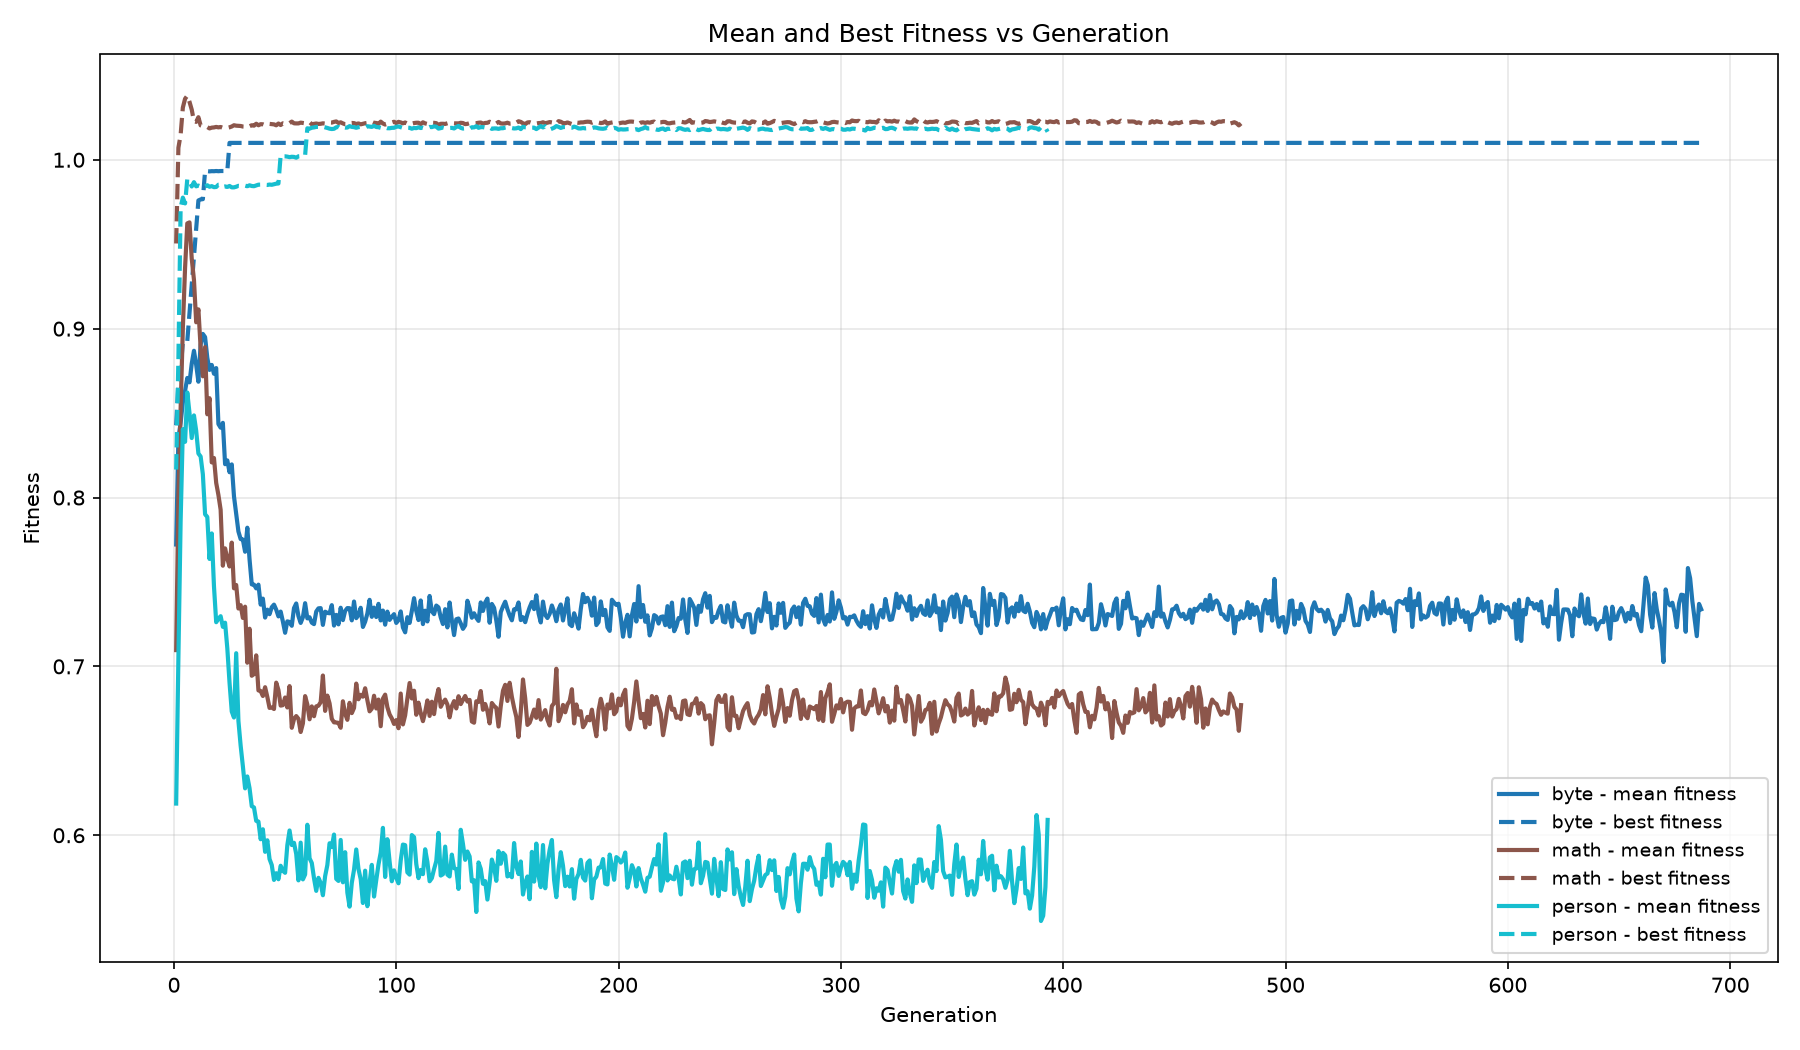
\includegraphics[width=\textwidth]{combined_fitness.png}
\caption{Mean and best fitness ($alpha=1.0$) for tests for each generation}
\label{fig:fig1}
\end{figure*}

This behavior directly motivates our work. In this ablation study, we investigate whether transforming FANDANGO's fitness calculation from a linear to a non-linear function (introducing an exponent value) can alter the search dynamics, improve the balance between exploration and exploitation, and ultimately lead to a more effective exploration of the solution space.


\section{Research question}\label{sec:res_quest}
Figure \ref{fig:fig1} shows a clear trend: after a sharp drop in early generations, the average fitness of the population plateaus at a relatively low level. This indicates that the fuzzer attempts to converge prematurely on initial solutions, favoring only a few individuals.

The fitness function $f:T\rightarrow \mathbb{R}$ is computed as shown in Equation (\ref{eq:fitness}):
\begin{align}\label{eq:fitness}
  f(T) = \left(\sum_{c\in C} w_c \cdot s_c(T)\right)^\alpha
\end{align}
where:
\begin{itemize}\item $w_c$ is the weight assigned to the constraint $c$.
\item $s_c \in [0,1]$ is the satisfaction score of the tree $T$ with respect to the constraint $c$.
\end{itemize}
As observed in Figure \ref{fig:fig1}, the total fitness values can exceed $1.0$. This occurs because FANDANGO's evaluator computes the final fitness as a cumulative sum of different constraint evaluations whose combined weights and scores are not strictly normalized to a global maximum of $1.0$. Since this behavior is inherent to the original fuzzer's implementation, we maintained it unchanged. This lack of strict normalization is not considered a problem for our study, as the non-linear transformation applied by $\alpha$ operates effectively on the relative fitness differences between individuals regardless of the absolute upper bound.

The described fitness equation, with the addition of the parameter $\alpha$, is the one used in this study. It is important to note that for $\alpha = 1.0$, the formula corresponds exactly to the original one described in the FANDANGO paper.
Specifically, this study addresses the following Research Question (\textit{RQ}): \textit{Does introducing a non-linear parameter ($\alpha$) in the fitness function improve FANDANGO's performance in terms of input validity and grammar coverage compared to the linear baseline ($\alpha=1.0$)}?

The introduction of the parameter $\alpha$ aims to directly influence the selection pressure within the genetic algorithm.
By mathematically compressing the gap between highly fit and poorly fit individuals, this transformation artificially expands the mutation pool. It relaxes the selection pressure, preventing the genetic algorithm from prematurely discarding suboptimal syntactic trees that might contain structural traits necessary to escape local optima.
In this study, we replicate the tests with different values of $\alpha$ (see Section \ref{sec:meth}) to extract information about how this approach alters the fuzzer's search and exploration behavior.



\section{Methodology} \label{sec:meth}
To effectively evaluate the impact of the non-linear fitness transformation, it was necessary to design a set of targeted benchmarks. The experimental evaluation in the original FANDANGO paper primarily utilized tests with relatively loose constraints. Consequently, the fuzzer often generated highly fit individuals right from the initial generations, rapidly saturating the fitness score and leaving little room to observe the evolutionary growth and the search dynamics over time.

To overcome this limitation and properly expose the effects of the parameter $\alpha$ on the selection pressure, we designed three custom tests. These tests were designed with different constraints types, intentionally making it difficult for the fuzzer to easily guess the optimal derivation trees. Each test targets a distinct data representation and structural challenge within the context-free grammar constraints.

\subsection{Benchmark Design}
The custom test suite consists of three distinct specification files:
\begin{itemize}
\item \textit{Test 1 (person):} The grammar defines a simple person record consisting of a name and an age. This scenario tests the algorithm's ability to satisfy numeric ranges and specific string patterns simultaneously. Each constraint is independent.
    \item \textit{Test 2 (math):} This scenario tests the fuzzer's capability to handle recursive grammar structures and semantic execution. The grammar generates arithmetic expressions composed of numbers, basic operators, and parentheses. This stresses the fuzzer's ability to navigate deep recursion while maintaining semantic validity.
    \item \textit{Test 3 (byte):} This test evaluates the generation of binary-like structures and global inter-dependencies. This represents a highly deceptive landscape for a genetic algorithm, as mutating a value might invalidate a dependent field and vice versa.
\end{itemize}

\subsection{Test Execution}
For test execution, a different approach compared to the original FANDANGO paper was chosen. Instead of executing long-running tests to achieve high grammar coverage and high solution number, we preferred to execute multiple short tests. This approach makes more sense for this study, since the goal is not to generate as many solutions as possible, but to study the fitness growth and solution validity percentage in the stochastic scenario of the evolution algorithm.

The executed tests evaluated different $\alpha$ values:
\begin{itemize}
\item $\alpha = 1.0$: Represents the baseline; it is the FANDANGO algorithm without any modification to the execution code
\item $\alpha = 0.5$: As described in Section \ref{sec:res_quest}, this aims to increase the average fitness value in order to discover new searching behaviors and try to expand the search space.
\item $\alpha = 2.0$: Used to penalize the mean fitness and reward best individuals.
\item $\alpha = 0.15$: Similarly to $\alpha = 0.5$, $\alpha=0.15$ is used to increase the fitness values further.
\end{itemize}


\subsection{Experimental Setup}
For each value of $\alpha$,  the three tests were performed 10 times for 10 minutes each, for a total of 300 minutes (5 hours) per configuration of $\alpha$ (with a total budget of 20 hours). Moreover, since genetic algorithms are stochastic, the same default parameters (such as population size, expected fitness, crossover rate, etc.) were adopted for each test.
In order to promote reproducibility, a deterministic seed was used and changed for each of the ten test runs.
Each time the output produced by FANDANGO was saved inside a list and the solution correctness was checked using a Python script (as done in the official paper tests).
Moreover, since FANDANGO utilizes some cache optimization in the evolution of the population, each test was isolated inside a dedicated process, in order to avoid memory sharing between executions that could affect other tests. 

Each test was executed with the following hardware specifications:
\begin{itemize}
\item AMD Ryzen 7 PRO dedicating 8 performance cores
  \item 32 GB of RAM
\end{itemize}
After the tests, some scripts were used to extract useful metrics for the comparison of the results.
  The source code, Python scripts, and raw experimental outputs are publicly available at:
\url{https://github.com/d4ni-02/FandangoFitnessStudy.git}.



\subsection{Evaluation Metrics}
Since different $\alpha$ values change the selection pressure of the evolutionary algorithm, fitness values (such as \textit{mean}, \textit{standard deviation} and the \textit{best} values) obtained with different $\alpha$ values are not directly comparable across different test configurations. For this reason in this study we will consider for the comparison some invariant metrics.
These are:
\begin{itemize}
\item \textit{valid solution percentage}: the percentage of valid inputs produced.
\item \textit{grammar coverage}: the obtained 4-path grammar coverage.
\item \textit{covered rules}: covered grammar rules during the evolution of the population.
\item \textit{Vargha-Delaney $\hat{A}_{12}$} and \textit{Mann-Whitney p-value}: to quantify differences between the $\alpha$ values.
\end{itemize}


\section{Results}
The obtained results for the valid solutions are reported in Table \ref{tbl:valid_solutions_all}, while the grammar coverage in Table \ref{tbl:grammar_coverage}. For the valid solution percentage, $\Delta_{Sol}$ expresses the relative variation in the number of valid solutions with respect to the baseline $\alpha=1.0$ and it is computed as in Equation (\ref{eq:delta}).
\begin{align}\label{eq:delta}
  \Delta_{Sol} = \frac{ValidSol_{\alpha} - ValidSol_{\alpha=1.0}}{ValidSol_{\alpha=1.0}}
\end{align}



\subsection{Valid Solutions}
For Test 1 (person), all non-linear configurations produce a positive $\Delta_{Sol}$, indicating that a modified fitness function can increase the number of valid solutions even when the grammar constraints are relatively simple. The largest improvement is obtained with $\alpha=0.15$, followed by $\alpha=2.0$, while $\alpha=0.5$ yields a more contained gain.

In Test 2 (math), only $\alpha=0.5$ shows a positive $\Delta_{Sol}$, whereas both $\alpha=0.15$ and $\alpha=2.0$ slightly reduce the number of valid solutions compared with the baseline.

Test 3 (byte) exhibits the strongest and most consistent response: all non-linear values improve the baseline, with $\alpha=0.5$ achieving the highest $\Delta_{Sol}$ and $\alpha=0.15$ closely following.

Overall, these trends suggest that the effect of the exponent is problem-dependent, but values with $\alpha<1$ tend to be beneficial, particularly in more complex and interdependent search spaces.


\begin{table*}[htbp]
  \centering
  \begin{tblr}{|l|l|l|l|l|}
    \hline
    Test & $\alpha$ & Valid solutions (mean $\pm$ std) & Valid percentage (\%) & $\Delta_{Sol}$ vs $\alpha=1.0$ \\
    \hline
    \SetCell[r=4]{l} Test 1\\(Person) 
      & 1.0 (baseline) & 475.9 $\pm$ 325.9 & 25.84 $\pm$ 15.41 & --- \\
      & 0.15           & 563.7 $\pm$ 224.9 & 29.21 $\pm$ 11.72 & $+18.4\%$ \\
      & 0.5            & 505.7 $\pm$ 385.5 & 25.61 $\pm$ 19.01 & $+6.3\%$ \\
      & 2.0            & 549.0 $\pm$ 291.8 & 28.16 $\pm$ 12.88 & $+15.4\%$ \\
    \hline
    \SetCell[r=4]{l} Test 2\\(Math)
      & 1.0 (baseline) & 876.1 $\pm$ 87.2  & 21.63 $\pm$ 2.79  & --- \\
      & 0.15           & 837.3 $\pm$ 129.5 & 20.75 $\pm$ 2.13  & $-4.4\%$ \\
      & 0.5            & 935.3 $\pm$ 97.7  & 23.33 $\pm$ 2.42  & $+6.8\%$ \\
      & 2.0            & 867.6 $\pm$ 84.4  & 22.12 $\pm$ 2.40  & $-1.0\%$ \\
    \hline
    \SetCell[r=4]{l} Test 3\\(Byte)
      & 1.0 (baseline) & 1440.5 $\pm$ 644.9 & 53.36 $\pm$ 15.32 & --- \\
      & 0.15           & 1845.6 $\pm$ 435.2 & 60.61 $\pm$ 12.29 & $+28.1\%$ \\
      & 0.5            & 1921.3 $\pm$ 743.2 & 62.82 $\pm$ 21.18 & $+33.4\%$ \\
      & 2.0            & 1652.1 $\pm$ 664.4 & 58.22 $\pm$ 21.04 & $+14.7\%$ \\
    \hline
  \end{tblr}
  \vspace{0.2cm}
  \caption{Valid Solutions across Benchmark Tests}
  \label{tbl:valid_solutions_all}
\end{table*}

The box plot in Figure \ref{fig:fig2} illustrates the distribution of valid solution percentages across the three benchmark subjects. The visual comparison reveals substantial overlap among the distributions for all $\alpha$ values within each subject. While Test 2  exhibits low variance, both Test 1 and Test 3 display high variability and susceptibility to noise, characterized by wide interquartile ranges. This observed dispersion directly supports the Mann-Whitney $p$-value results discussed in Section \ref{sec:stats}, confirming the absence of statistically significant performance differences across the evaluated configurations.

\begin{figure*}[htbp]
\centering
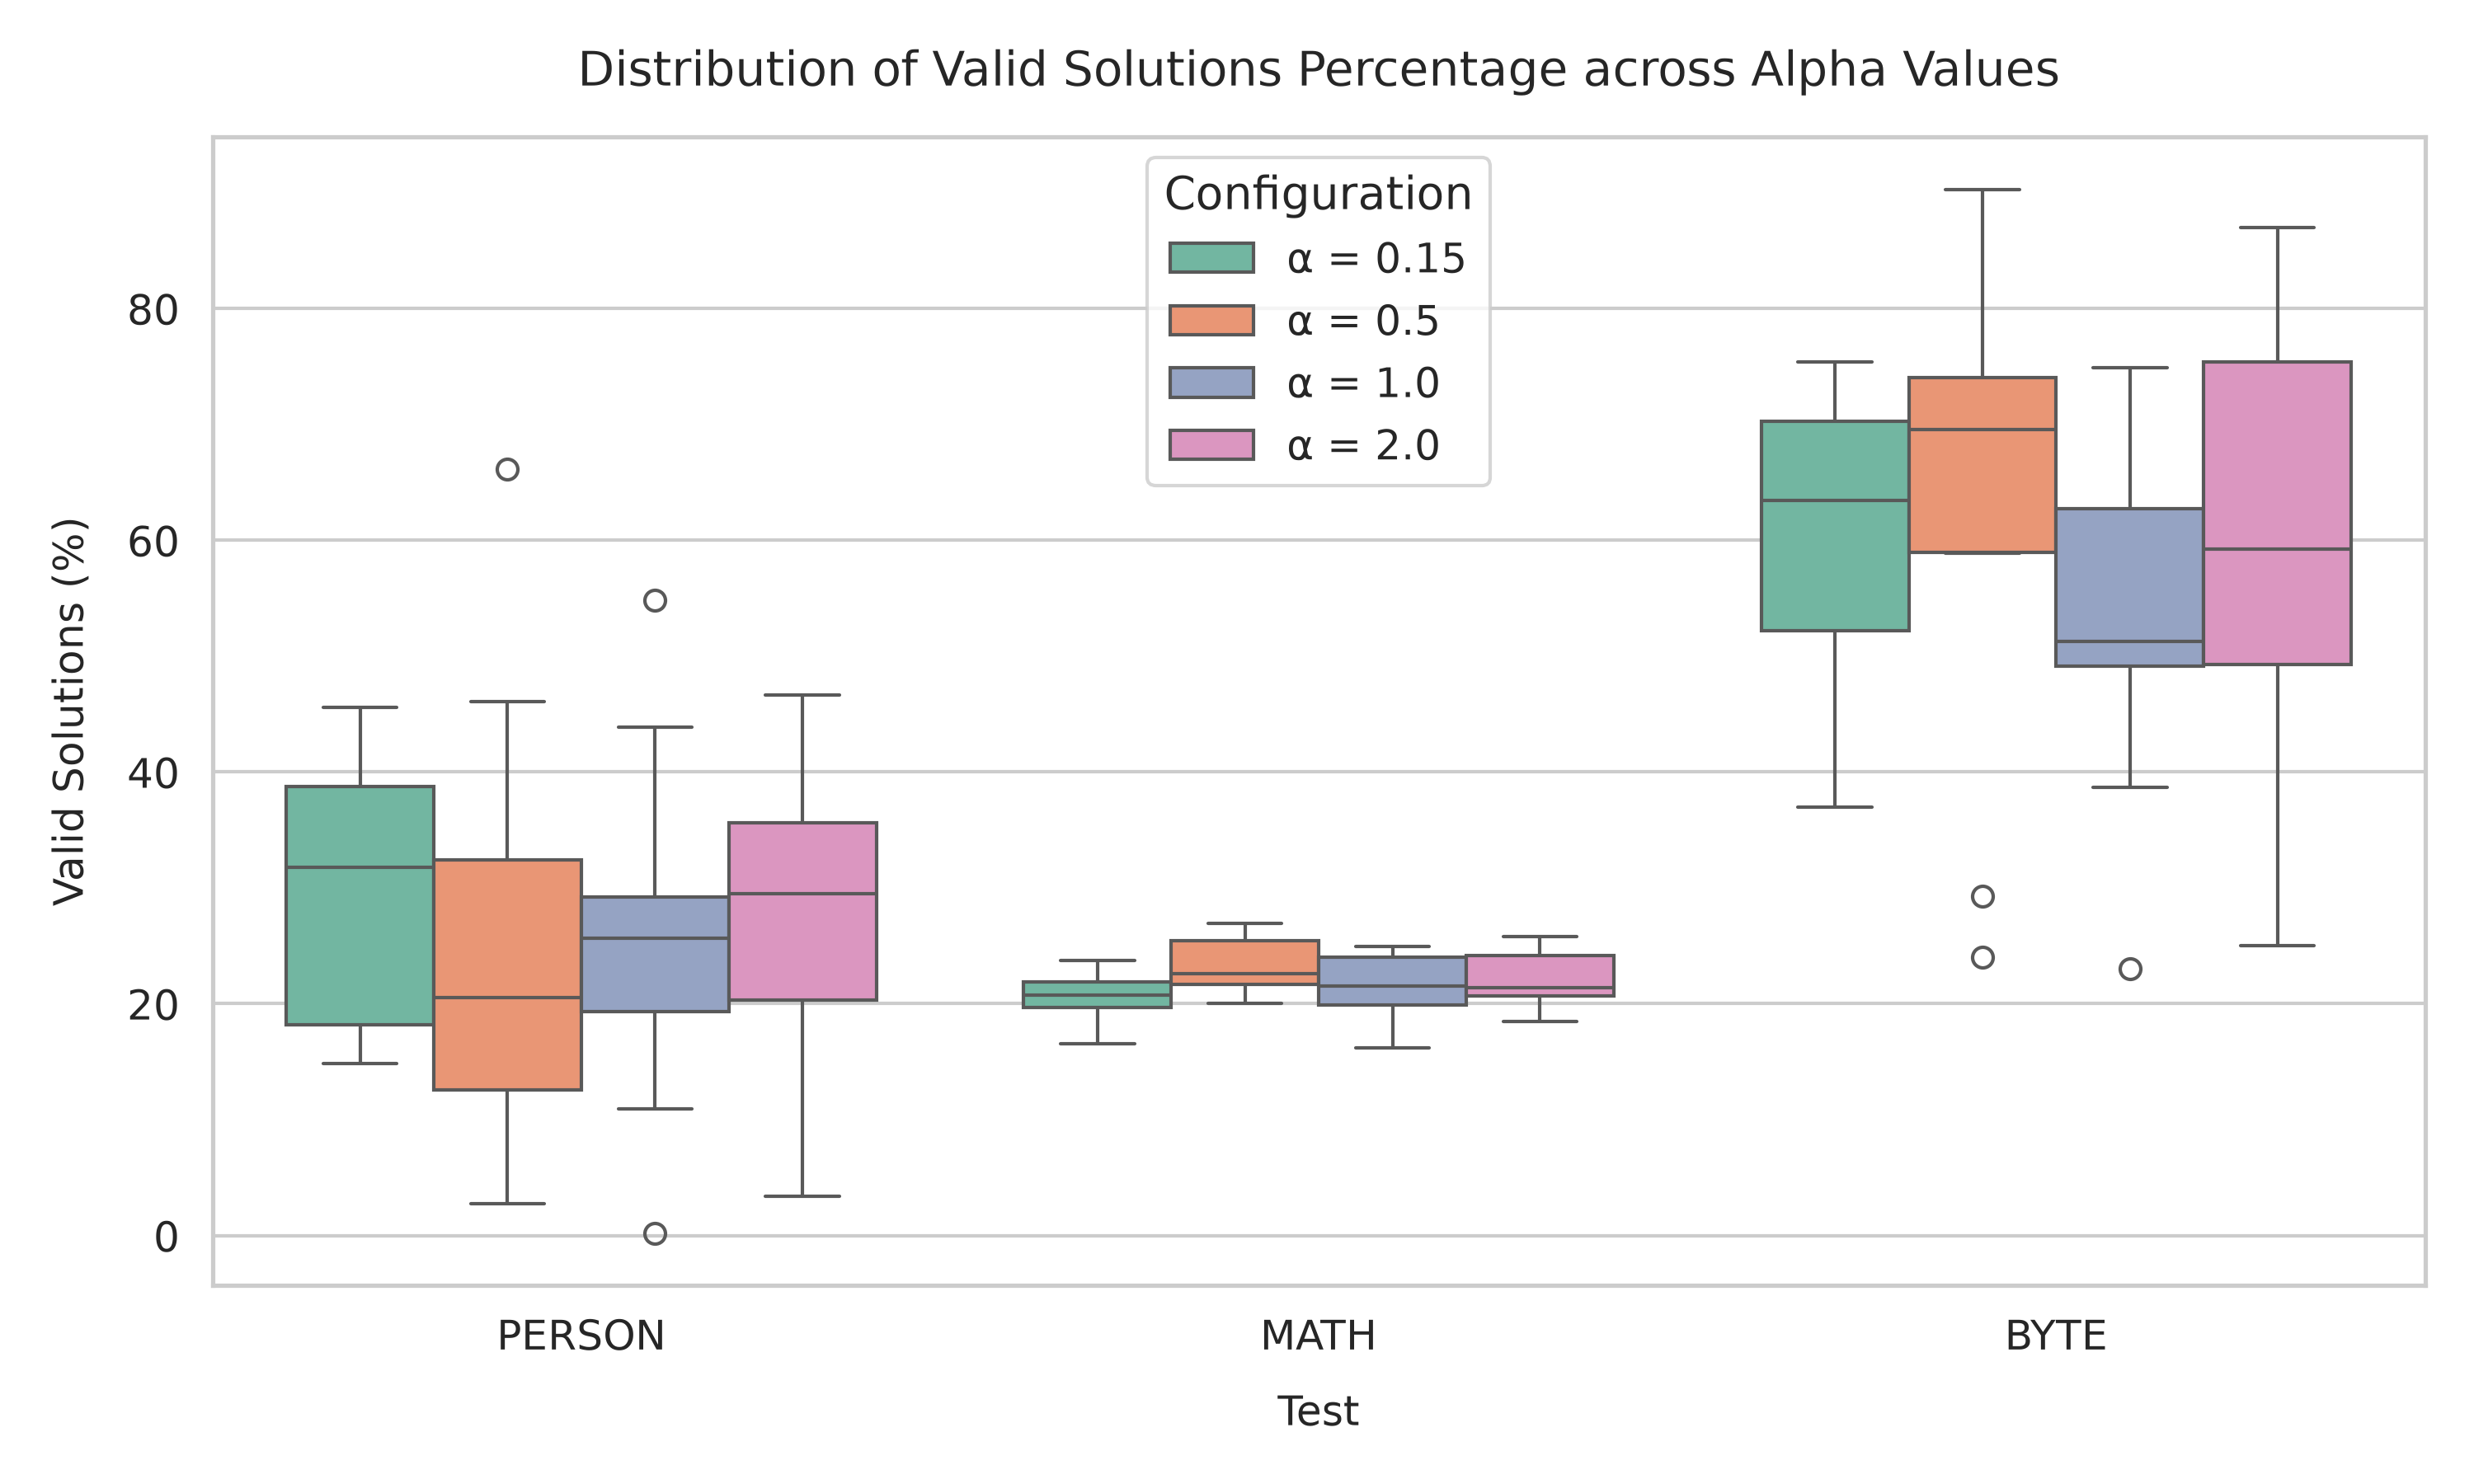
\includegraphics[scale=.6]{valid_solutions_boxplot.png}
\caption{Valid solution mean for each test}
\label{fig:fig2}
\end{figure*}


\subsection{Grammar Coverage}
The mean grammar coverage percentages across all test configurations are summarized in Table \ref{tbl:grammar_coverage}. 

For Test 1 (person), lower values of $\alpha$ increase average grammar coverage, reaching a peak of $100\%$ with $\alpha=0.15$ (compared to $94.30\%$ for the baseline), accompanied by an increase in the mean number of covered rules from $327.2$ to $373.2$. This indicates that expanding the mutation pool helps the search process discover previously unexplored grammatical branches.

In Test 2 (math), grammar coverage remains virtually unaffected by changes in $\alpha$ (with a constant average of $109.0$ covered rules), demonstrating that recursive grammar structures are structurally resilient to adjustments in fitness pressure.

In Test 3 (byte), non-linear configurations lead to a slight reduction in grammar coverage (dropping from $51.25\%$ to approximately $48.5\%$, with covered rules decreasing slightly from $24.6$ to $\approx 23.3$), despite generating a higher percentage of valid solutions. This highlights a subtle trade-off: reducing selection pressure aids in satisfying complex structural constraints but may slightly confine overall grammar exploration.

\begin{table*}[htbp]
  \centering
  \begin{tblr}{|l|c|c|c|}
    \hline
    $\alpha$ & Test 1 (Person) (\%) & Test 2 (Math) (\%) & Test 3 (Byte) (\%) \\
    \hline
    1.0 (baseline) & 94.30 & 36.19 & 51.25 \\
    \hline
    0.15           & 100.00 & 36.33 & 48.75 \\
    \hline
    0.5            & 100.00 & 36.33 & 48.54 \\
    \hline
    2.0            & 95.56  & 35.33 & 48.33 \\
    \hline
  \end{tblr}
  \vspace{0.2cm}
  \caption{Mean grammar coverage percentage across tests.}
  \label{tbl:grammar_coverage}
\end{table*}


\subsection{Vargha-Delaney $\hat{A}_{12}$ and Mann-Whitney $p$-value} \label{sec:stats}
To evaluate the practical significance of the non-linear fitness variants relative to the linear baseline, we calculated the Vargha-Delaney $\hat{A}_{12}$ \cite{vargha2000critique} non-parametric effect size metric. In our setup, $\hat{A}_{12}$ represents the probability that a randomized run from a specific non-linear configuration yields a higher percentage of valid solutions than a run from the standard linear baseline. 

An $\hat{A}_{12}$ score of $0.50$ indicates stochastic equivalence between the two algorithms. Values above $0.50$ favor the non-linear configuration, with conventional thresholds categorizing the effect size magnitude as small ($\hat{A}_{12} > 0.56$), medium ($\hat{A}_{12} > 0.64$), or large ($\hat{A}_{12} > 0.71$). Conversely, values below $0.44$ indicate that the linear baseline outperforms the non-linear variant.

Table \ref{tbl:a12_scores} summarizes the computed $\hat{A}_{12}$ effect sizes and the Mann-Whitney $p$-values \cite{mann1947test} across all benchmark tests.
We did not observe statistically significant differences between the $\alpha$ variants and the linear baseline on any subject (all $p > 0.18$, Mann-Whitney U test). The effect sizes ranged from small to medium, without a consistent pattern across subjects. This indicates that the observed variations are compatible with random noise, and current data are insufficient to claim the superiority of any specific configuration.

\begin{table*}[htbp]
  \centering
  \begin{tblr}{|l|l|c|c|}
    \hline
    Test & Configuration & $\hat{A}_{12}$ Score & p-value \\
    \hline
    Test 1 (Person) & $\alpha = 0.15$ vs Linear & 0.58 & 0.5708\\
                    & $\alpha = 0.5$ vs Linear  & 0.46 & 0.7913\\
                    & $\alpha = 2.0$ vs Linear  & 0.59 & 0.5205\\
    \hline
    Test 2 (Math)   & $\alpha = 0.15$ vs Linear & 0.38 & 0.3847\\
                    & $\alpha = 0.5$ vs Linear  & 0.67 & 0.2123\\
                    & $\alpha = 2.0$ vs Linear  & 0.56 & 0.6776\\
    \hline
    Test 3 (Byte)   & $\alpha = 0.15$ vs Linear & 0.65 & 0.2730\\
                    & $\alpha = 0.5$ vs Linear  & 0.68 & 0.1859 \\
                    & $\alpha = 2.0$ vs Linear  & 0.61 & 0.4274 \\
    \hline
  \end{tblr}
  \vspace{0.2cm}
  \caption{Vargha-Delaney $\hat{A}_{12}$ effect size for valid solutions relative to the baseline ($\alpha=1.0$).}
  \label{tbl:a12_scores}
\end{table*}





\section{Conclusion}
In this study, we presented an ablation analysis investigating the impact of a non-linear fitness function on the FANDANGO fuzzer. By introducing an exponent parameter $\alpha$ into the fitness evaluation, we altered selection pressure to observe how relaxed or intensified scaling affects valid input generation and grammar coverage dynamics.

While descriptive averages suggest that reducing selection pressure may visually appear to increase the yield of valid solutions in specific complex domains (such as Test 3), these differences are not statistically significant. Similarly, the impact on grammar coverage remains domain-dependent: lower $\alpha$ values expanded coverage in simpler grammars, coverage remained invariant in recursive settings, and exhibited a slight decrease in highly constrained inter-dependent structures. As shown by the $p$-value computations (Table~\ref{tbl:a12_scores}), the observed variations remain compatible with random noise.

Consequently, this work should be interpreted as a pilot study providing preliminary insights into fitness function tuning for evolutionary grammar fuzzing.




\section{Limitations and Future Work}
The primary limitation of this study lies in the experimental budget trade-off. We conducted 10 independent runs of 10 minutes for each configuration and test, totaling 20 hours of total computation. This design prioritized a high number of independent repetitions to capture early population evolution and accurately estimate variance, rather than long-term convergence.

However, genetic algorithms and fuzzers are inherently stochastic processes where short time windows amplify variance and restrict the analysis to early evolutionary phases. This trade-off limits the ability to observe low-probability structural mutations that may emerge only after longer evolutionary periods. Therefore, the absence of statistically significant differences should not be interpreted as evidence that $\alpha$ has no effect, but rather that the current experimental setup lacks the statistical power to detect subtle or long-term dynamics.

Future work will address these limitations by executing longer test runs (e.g., 1 hour or more) across a larger set of deterministic seeds, enabling the evolutionary algorithm to approach asymptotic behavior. Furthermore, since optimal selection pressure appears to depend heavily on the target grammar's structure, a promising research direction is the implementation of a dynamic or adaptive $\alpha$ mechanism. Such an approach could dynamically adjust selection pressure during execution, for instance, initializing with lower $\alpha$ values to encourage early exploration before gradually increasing pressure during exploitation.






\FloatBarrier
\bibliographystyle{IEEEtran}
\bibliography{references}





\end{document}
